\label{sec:aggregating}

We denote by \kastarphi the instantiation of \kastar that uses a given aggregation function $\Phi$. In the rest of this section, we examine under which assumptions on $\Phi$ and on the heuristics $\vect{h}$ we can obtain optimality guarantees on \kastarphi.
As we shall see, there is a tradeoff between the two types of assumptions: making stronger assumptions on the heuristics leads to a
larger class of aggregation functions that guarnatee optimality. %optimality for a larger range of aggregation functions. [[AF: not sure what the sentence means: it means optimallity]][[AS: Better now?]

Before analyzing the different aggregation functions and heuristics,  we provide the following definitions and invariant which holds in \kastar regardless of how the heuristics and $\Phi$ are computed.

\begin{definition}
  An algorithm for the \kgs is \emph{admissible} if in any instance, for all reachable goals $t_i$, the first path found to $t_i$ is optimal.
  An algorithm for the \kgs is \emph{$1$-admissible} if in any instance, there exists a goal $t_i$ such that the first path found to $t_i$ is optimal.
  [[Roni: do we need this 1-admissible? I rather we called this admissible]]
\end{definition}
\abda{check 1-admissible definition in case some goals are not reachable}

Since we defined \kgs for graphs with non-negative edge costs, we limit the discussion to non-negative heuristic functions and correspondingly heuristic aggregation functions that accept non-negative values. Formally,   
\begin{definition}
  Let $k$ be a fixed positive integer.
  A \emph{heuristic aggregation function} is a function $\Phi: \nonnegreals^k \rightarrow \nonnegreals$ such that $\Phi(\vect{0}) = 0$, where $\vect{0}$ is the $k$-dimensional zero vector.
\end{definition}

\begin{lemma}
  \label{lem:simple}
  In every iteration of \kastar, for every active goal $t_i$, there exists a state $n$ in \open on an optimal path to $t_i$, i.e., $g(n) + d(n, t_i) = d(s, t_i)$.
\end{lemma}

Lemma~\ref{lem:simple} can be proven by induction over the iterations of \kastar.
Namely, it trivially holds in the first iteration and continues to hold in subsequent iterations because when a node with $g(\cdot) + d(s,\cdot) = d(s, t_i)$ is expanded then one of its children must also have $g(\cdot) + d(s,\cdot) = d(s, t_i)$.
An equivalent to Lemma~\ref{lem:simple} has been proven for many other best-first search algorithms.

\begin{lemma}[Completeness]
  \label{lem:completeness}
  If a goal is reachable, then it is eventually expanded by \kastar. 
  %[[AF: but not necessarily optimal]
\end{lemma}
Note that Lemma~\ref{lem:completeness} does not say that the optimal path to each goal will be found. This requires some restrictions over the heuristics and aggregation function used, as we discuss next. 

\subsection{Consistent Heuristics}

We begin our exploration by considering the case where all heuristic functions are \emph{consistent} (Definition~\ref{def:consistent}). 


\begin{definition}
A heuristic aggregation function $\Phi$ is \emph{\axiomcons} iff for every vectors $\vect{v}$ and $\vect{u}$, we have that if there exists $i$ such that  $u_i = 0$ then $\Phi(\vect{v}) - \Phi(\vect{u}) \leq \max (\vect{v}-\vect{u})$.
\end{definition}
By $u_i$ we refer the $i^{th}$ element in $\vect{u}$. 

%\abda{Alternative names: \emph{metric}, \emph{weak contraction}. See \url{https://en.wikipedia.org/wiki/Metric_map} for inspiration.}
% Similar to \cite{Denardo1967}

\begin{theorem}
  \label{thm:consistent}
  Let $\Phi$ be a \axiomcons heuristic aggregation function.
  For any \kgs and for any tuple of consistent heuristics $\vect{h}$, \kastarphi is $k$-admissible.
\end{theorem}
\begin{proof}
  Assume that \kastar chooses to expand a goal $t_i \in \{t_1, \ldots t_k\}$) via a path $p$. 
  Applying Lemma~\ref{lem:simple} to $t_i$, we obtain there exists $n\in \open$ such that $g(n) + d(n, t_i) = d(s, t_i)$.
  Since $t_i$ is expanded before $n$, we have 
  \begin{equation}
      g(t_i) + \Phi(\vect{h}(t_i)) = F(t_i) \leq F(n) = g(n) + \Phi(\vect{h}(n))
  \end{equation}
    Since all heuristics are consistent, we have that for every $j$
  \begin{align}
    h_j(n)                  & \leq d(n, t_i) + h_j(t_i)   \\
    h_j(n) - h_j(t_i)       & \leq d(n, t_i)               
%    \Phi(\vect{h}(n)) - \Phi(\vect{h}(t_i)) & \leq d(n, t_i) & \text{($\Phi$ is \axiomcons and $h_i(t_i) = 0$)}\\
\end{align}
Since this holds for every $j$, we have: 
\begin{align}
    \max (\vect{h}(n) - \vect{h}(t_i)) & \leq d(n, t_i)              & \text{}\\
    \Phi(\vect{h}(n))-\Phi(\vect{h}(t_i))  & \leq d(n, t_i)  & \text{($\Phi$ is \axiomcons and $h_i(t_i) = 0$)}\\
        \Phi(\vect{h}(n))  & \leq d(n, t_i) + \Phi(\vect{h}(t_i)) & \\
    g(n) + \Phi(\vect{h}(n))           & \leq g(n)+ d(n, t_i) + \Phi(\vect{h}(t_i)) & \\
    F(n)           & \leq d(s, t_i) + \Phi(\vect{h}(t_i)) &
    \text{($n$ is chosen via Lemma~\ref{lem:simple})}
  \end{align}  
    Now, since $t$ is expanded before $n$, we have that $F(t_i) \leq F(n)$. 
  \begin{align}  
    F(t_i) \leq F(n)                     & \leq d(s, t_i) + \Phi(\vect{h}(t_i)) & \text{($t_i$ is expanded before $n$)}\\
    g(t_i) + \Phi(\vect{h}(t_i))           & \leq d(s, t_i) + \Phi(\vect{h}(t_i)) & \text{(by definition of $F$)}\\
    g(t_i)                & \leq d(s, t_i) & 
    \label{eq:consistent}
  \end{align}
  By definition of $d$, we know that $d(s,t_i)\leq g(t_i)$. Therefore, when we expand a goal its $g$ value is equal to $d(s, t_i)$ as required.
\end{proof}

Theorem~\ref{thm:consistent} shows that being \axiomcons is a sufficient condition for optimality of \kastarphi with consistent heuristics.
Our next result shows that it is a necessary condition. 
\begin{figure}
  \centering
  \subfloat{
  \begin{tikzpicture}
    \node[source] (s) at (0, 2) {$S$};
    \node[other]  (a) at (4, 2) {$A$};
    \node[target1] (b) at (4, 0) {$B$};
    \node[target2] (c) at (0, 0) {$C$};

    \draw[->] (s) -- (a) node[midway] (sa) {\phantom{0}};
    \draw[->] (s) -- (b) node[midway] (sb) {\phantom{0}};
    \draw[->] (s) -- (c) node[midway] (sc) {\phantom{0}};
    \draw[->] (a) -- (b) node[midway] (ab) {\phantom{0}};

    \node[above = -2mm of sa,edgeweight] {$\epsilon$};
    \node[below left = -5mm of sb,edgeweight] {$\delta + 2\epsilon$};
    \node[left  = -2mm of sc,edgeweight] {$\Phi(\vect{v})$};
    \node[right = -2mm of ab,edgeweight] {$\delta$};

    \node[left  = 2mm of  s,infobox] {$\vect{h}=\vect{0}$};
    \node[right = 2mm of  a,infobox] {$\vect{h}=\vect{v}$};
    \node[right = 2mm of  b,infobox] {$\vect{h}=\vect{u}$};
    \node[left  = 2mm of  c,infobox] {$\vect{h}=\vect{0}$};
  \end{tikzpicture}
  } \hfill
  \subfloat{
    \begin{tabular}[b]{lccc}
      \toprule
      Path & $g$ & $\Phi(\vect{h})$ & $F$\\
      \midrule
      $SB$ & $\delta + 2\epsilon$ & $\Phi(\vect{u})$ & $\Phi(\vect{v}) - \epsilon$ \\
      $SC$ & $\Phi(\vect{v})$ & $0$ & $\Phi(\vect{v})$\\
      $SA$ & $\epsilon$ & $\Phi(\vect{v})$ & $\Phi(\vect{v}) + \epsilon$ \\
      $SAB$ & $\delta + \epsilon$ & $\Phi(\vect{u})$ & $\Phi(\vect{v}) - 2\epsilon$ \\
      \bottomrule
    \end{tabular}
  }
  \caption[Generic counter-example for \kastarphi]{Generic counter-example for \kastarphi. 
  The start is $S$, $B$ is the $i$\textsuperscript{th} goal, and $C$ is the $j$\textsuperscript{th} goal for $j \neq i$. 
  For any, $\vect{v}$, $\vect{u}$, $i$, $\delta$, and $\epsilon$ such that (1) $u_i = 0$, (2) $\delta > 0$, (3) $\Phi(\vect{v}) > \Phi(\vect{u}) + \delta$, and (4) $\epsilon = \frac{\Phi(v) - \Phi(\vect{u}) - \delta}{3} > 0$, running \kastarphi will return a suboptimal path to $B$. 
  
  To see this, the table on the right shows the $g$, $\Phi(\vect{h})$, and $F$ values for the possible paths to the graph nodes.
  The search expands $S$, $B$, $C$, then stops.
  The optimal path to $B$ is $SAB$, but \kastarphi returns the suboptimal path $SB$.}
  \label{fig:kstarphi-bad}
\end{figure}
\begin{theorem}
  \label{thm:consistent-dual}
  If a heuristic aggregation function $\Phi$ is not \axiomcons, then there exists a \kgs and a tuple of consistent heuristics such that \kastarphi is not $k$-admissible.
\end{theorem}
\begin{proof}
Since $\Phi$ is not \axiomcons, there exists vectors $\vect{v}$, $\vect{u}$, and an index $i$ such that $u_i = 0$ and $\Phi(\vect{v}) - \Phi(\vect{u}) > \max (\vect{v} - \vect{u})$. 
  Let $\delta$ such that $\Phi(\vect{v}) - \Phi(\vect{u}) > \delta > \max (\vect{v} - \vect{u})$.
Since the domain of $\Phi$ is vectors of non-negative values, $v_i \geq 0$ and so $\max (\vect{v} - \vect{u}) \geq v_i - u_i \geq 0$, therefore $\delta > 0$.


  Define $\epsilon = \frac{\Phi(\vect{v}) - \Phi(\vect{u}) - \delta}{3} > 0$.
  Using $\vect{v}$, $\vect{u}$, $i$, $\delta$, and $\epsilon$, we can construct a counter-example showing that \kastarphi is not $k$-admissible. 
  This counter example is given in Figure~\ref{fig:kstarphi-bad}. 
$S$ is the start, $B$ is the $i$\textsuperscript{th} goal and $C$ is the $j$\textsuperscript{th} goal for $j \neq i$. 
     As can be seen from the table above right, the search expands $S$, $B$, $C$, then stops. 
     The optimal path to $B$ is $SAB$, but \kastarphi returns the suboptimal path $SB$. 

  To conclude the proof, it remains to observe that the heuristics involved are consistent.
  This is indeed the case because for all $j$, we have $h_j(A) - h_j(B) = v_j - w_j \leq \max (\vect{v} - \vect{w}) < \delta = d(A, B)$ and therefore $h_j(A) \leq d(A, B) + h_j(B)$.
\end{proof}

[[UP TO HERE 19.10]]

Theorem~\ref{thm:consistent} opens the opportunity to run \kastar for a larger range of heuristic aggregation functions than Theorem~\ref{thm:admissible}, provided the heuristic functions are consistent.

\begin{observation}
  Any \axiomadm function is also \axiomcons.
%  In particular $\Phi=\min$ is \axiomcons.
\end{observation}
\begin{proof}
  Let $\Phi$ be an \axiomadm heuristic aggregation function and let $\vect{v}$ and $\vect{w}$ be vectors such that $\exists i, w_i = 0$.
  On the one hand, $\Phi(\vect{v}) - \Phi(\vect{w}) \leq \Phi(\vect{v}) \leq \min \vect{v} \leq v_i$.
  On the other hand, we have $w_i = 0$ so we derive $v_i \leq v_i - w_i \leq \max (\vect{v} - \vect{w})$.
  As result, $\Phi(\vect{v}) - \Phi(\vect{w}) \leq \max (\vect{v} - \vect{w})$, and we conclude that $\Phi$ is \axiomcons.
\end{proof}

Let $\{ v_i \}$ be a collection of terms. [[AF: what does that mean? numbers? Who is i? do you have vi, v2 etc?]][[AF: do you want to start a new definition here?]]
A \emph{subconvex} combination of these terms is a linear combination $\sum_i \alpha_i t_i$ where all coefficients are non-negative, $0 \leq \alpha_i$, and the sum of coefficients is no more than one, $\sum_i \alpha_i \leq 1$.

The $i$th \emph{order statistic} of a vector $\vect{v}$ is the $i$th smallest value of $\vect{v}$ and is denoted $v_{(i)}$. [[AF: why not just call it i'th smallest?]
For instance, if $\vect{v} = \tuple{3, 1, 0, 1}$, then $v_{(1)} = v_3 = 0$, $v_{(2)} = v_{(3)} = v_2 = v_4 = 1$ and $v_{(4)} = v_1 = 3$. [[AF: this is just a permutation along the values]

[[AF: jumped further. I am happy to sit down with whoever wrote this to further polish the text]

The \axiomcons axiom is not only as general as \axiomadm, but it also allows for aggregation functions not covered by the previous assumption:
\begin{theorem}
  \label{thm:subconvex}
  Subconvex combinations of the components and the order statistics give rise to \axiomcons heuristic aggregation functions.
\end{theorem}
\begin{proof}
  Consider $2k$ non-negative coefficients $\alpha_i$ such that $\sum_{1 \leq i \leq 2k} \alpha_i \leq 1$.
  Then, we will show that $\Phi$ defined as $\Phi(\vect{v}) = \sum_{1 \leq i \leq k} \alpha_i v_i + \alpha_{k+i} v_{(i)}$ is a heuristic aggregation function.
  For any two vectors $\vect{v}$ and $\vect{w}$, we have $\Phi(\vect{v}) - \Phi(\vect{w}) = \sum_{1 \leq i \leq k} \alpha_i (v_i - w_i) + \alpha_{(i+k)} (v_{(i)} - w_{(i)})$.
  On the one hand, $v_i - w_i \leq \max (\vect{v} - \vect{w})$ is direct, on the other hand, $v_{(i)} - w_{(i)} \leq \max (\vect{v} - \vect{w})$ can be established with a little bit more effort:

  Indeed, for $1 \leq i \leq k$, define $V_i = \{j, v_j < v_{(i)} \}$ and $W_i = \{j, w_j < w_{(i)} \}$ and observe that $|V_i| \leq i - 1$ and $|W_i| \leq k - i$ by definition of the order statistics.
  It follows that $|V_i \cup W_i| \leq k - 1$.
  From a counting argument, obtain an integer $1 \leq l_i \leq k$ such that $l_i \notin V_i \cup W_i$.
  By construction of $V_i$ and $W_i$, deduce that $v_{(i)} \leq v_{l_i}$ and that $w_{l_i} \leq w_{(i)}$ and conclude that $v_{(i)} - w_{(i)} \leq v_{l_i} - w_{l_i} \leq \max (\vect{v} - \vect{w})$.

  As a result, we have $\Phi(\vect{v}) - \Phi(\vect{w}) \leq \sum_{1 \leq i \leq 2k} \alpha_i \max(\vect{v} - \vect{w})$ because for all $i$, $\alpha_i$ is non-negative.
  Therefore, $\Phi(\vect{v}) - \Phi(\vect{w}) \leq \max(\vect{v} - \vect{w}) \sum_i \alpha_i \leq \max(\vect{v} - \vect{w})$, thus showing that $\Phi$ is \axiomcons.
\end{proof}

\begin{corollary}
  Using any of the \emph{mean}, the \emph{maximum}, the \emph{minimum}, the \emph{$i$th projection}, for $1 \leq i \leq k$, or the \emph{median} of the values in $\vect{v}$ gives a \axiomcons heuristic aggregation function.
\end{corollary}
\begin{proof}
  All these quantities can be expressed as subconvex combinations of the components and the order statistics, so they are all \axiomcons:
  The $i$th projection is $\Phi(\vect{v}) = v_i$; the \emph{mean} is $\Phi(\vect{v}) = \frac{v_1 + \dots + v_k}{k}$; the \emph{maximum} is $\Phi(\vect{v})= v_{(k)}$; the \emph{minimum} is $\Phi(\vect{v}) = v_{(1)}$; and the \emph{median} is $\Phi(\vect{v}) = \frac{1}{2}(v_{(\frac{k}{2})} + v_{(\frac{k+1}{2})})$.
\end{proof}

It is easy to show that for $2 \leq k$, none of these heuristic aggregation function is \axiomadm, except for the \emph{minimum}.
Thus, Theorem~\ref{thm:consistent} does indeed extend the range of functions for which we can obtain guarantees to other natural aggregation methods.

\begin{observation}
  The following heuristic aggregation functions do not satisfy \axiomcons.
  The \emph{sum} aggregation, $\Phi(\vect{v}) = \sum_i v_i$ is not \axiomcons as soon as there are two goals or more.
  More generally, combinations of the components that are not subconvex do \emph{not} give rise to \axiomcons heuristic aggregation functions.
\end{observation}
\begin{proof}
  Consider non-negative coefficients $\alpha_i$ such that $\sum_i \alpha_i > 1$.
  Then, $\Phi$ defined as $\Phi(\vect{v}) = \sum_i \alpha_i v_i$ is a heuristic aggregation function.
  However, taking for instance $\vect{v} = \vect{1}$ and $\vect{w} = \vect{0}$, we have $\vect{v} - \vect{w} = \sum_i \alpha_i (1 - 0) = \sum_i \alpha_i > 1 = \max (\vect{v} - \vect{w})$.
  Therefore $\Phi$ is not \axiomcons.
  In particular, the sum aggregation function is not \axiomcons.
\end{proof}

\begin{observation}
  The \emph{range statistic}, $\Phi(\vect{v}) = v_{(k)} - v_{(1)}$, is \axiomcons.
  For $k \geq 3$, the ``almost-range'' statistic defined as $\Phi(\vect{v}) = v_{(k)} - v_{(2)}$ is not \axiomcons.
\end{observation}
\begin{proof}
\abda{blabla}
\end{proof}

%\subsection{blabla}

\begin{theorem}
  \label{the:kastarmin-surplus}
  For any \kgs and for any tuple of consistent heuristics $\vect{h}$, \kastarmin never expands a surplus state.
\end{theorem}
\begin{proof}
  Let $n$ be a node expanded by \kastarmin.
  Let $t_i$ be such that $h_{t_i}(n) = \min h_{t_i}(n)$.
  Applying Lemma~\ref{lem:simple} to $t_i$, we obtain $n_i \in \open$ such that $g(n_i) + d(n_i, t_i) = d(s, t_i)$.
  For any node $p$ on the path from $s$ to $n$, we have the following derivation.
  \begin{align}
    h_{t_i}(p)        & \leq d(p, n) + h_{t_i}(n)         & \text{($h_{t_i}$ is consistent)}\\
    h_{t_i}(p)        & \leq d(p, n) + \Phi(\vect{h}(n))         & \text{(from the choice of $t_i$)}\\
    g(p) + h_{t_i}(p) & \leq g(p) + d(p, n) + \Phi(\vect{h}(n)) & \text{}\\
    g(p) + h_{t_i}(p) & \leq g(n) + \Phi(\vect{h}(n))          & \text{Lemma blabla}\\
    g(p) + h_{t_i}(p) & \leq F(n)         & \text{(by definition of $F$)}\\
    g(p) + h_{t_i}(p) & \leq F(n_i) = g(n_i) + \Phi(\vect{h}(n_i))      & \text{($n$ is expanded)}\\
    g(p) + h_{t_i}(p) & \leq g(n_i) + h_i(n_i) & \text{(by definition of $\Phi$)}\\
    g(p) + h_{t_i}(p) & \leq g(n_i) + d(n_i, t_i) & \text{($h_{t_i}$ is admissible)}\\
    g(p) + h_{t_i}(p) & \leq d(s, t_i) & \text{($n_i$ is chosen via Lemma~\ref{lem:simple})}
    \label{eq:nosurplus}
  \end{align}
  Thus, $n$ is not surplus for the SPP $\Pi_i$.
  Therefore, $n$ is not surplus for the \kgs.
\end{proof}

Note that our assumption that $h_{t_1}, \ldots h_{t_k}$ are consistent is necessary for the proof of Theorem~\ref{the:kastarmin-surplus}.
With an admissible but inconsistent heuristic, \kastarmin may, in fact, expand surplus states.
Figure~\ref{fig:inconsistent} shows a \kgs problem with $k = 2$ where this occurs.
\kastarmin will expand all states in the figure, while $B$ is surplus for both goals.

\begin{figure}
%  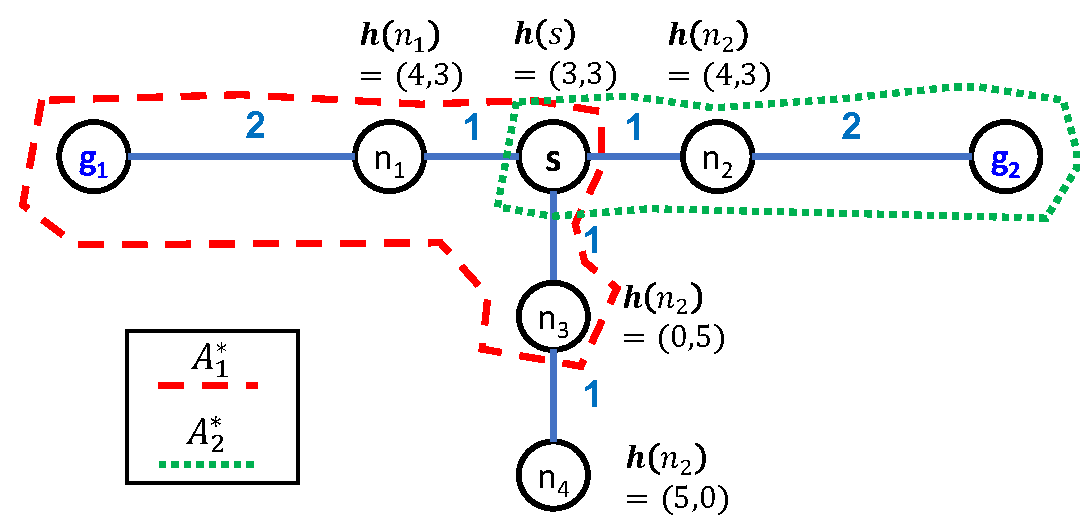
\includegraphics[width=\columnwidth]{inconsistent_cropped.pdf}
  \subfloat{
    \begin{tikzpicture}
    \node[source]  (s)  at (0, 2) {$S$};
    \node[other]   (a)  at (2, 0) {$A$};
    \node[other]   (b)  at (4, 0) {$B$};
    \node[target1] (t1) at (0, 0) {$t_1$};
    \node[target2] (t2) at (3, 2) {$t_2$};

    \draw[->] (s) -- (a)  node[midway] (sa) {\phantom{0}};
    \draw[->] (a) -- (b)  node[midway] (ab) {\phantom{0}};
    \draw[->] (s) -- (t1) node[midway] (st1) {\phantom{0}};
    \draw[->] (s) -- (t2) node[midway] (st2) {\phantom{0}};

    \node[above right = -5mm of sa,edgeweight] {$1$};
    \node[above = -2mm of ab,edgeweight] {$1$};
    \node[left  = -2mm of st1,edgeweight] {$3$};
    \node[above = -2mm of st2,edgeweight] {$3$};

    \node[above = 1mm of  s,infobox] {$\vect{h}=\vect{0}$};
    \node[below = 0mm of  a,infobox] {$\vect{h}=\tuple{0, 5}$};
    \node[below = 0mm of  b,infobox] {$\vect{h}=\tuple{5, 0}$};
    \node[below = 1mm of  t1,infobox] {$\vect{h}=\tuple{0, 5}$};
    \node[above = 0mm of  t2,infobox] {$\vect{h}=\tuple{5, 0}$};
  \end{tikzpicture}
  } \hfill
  \subfloat{
    \begin{tabular}[b]{l*8{c}}
      \toprule
      \multirow{2}{*}{Path} &     & \multicolumn{2}{c}{\astari{t_1}} & \multicolumn{2}{c}{\astari{t_2}} & \multicolumn{3}{c}{\kastarmin} \\
      \cmidrule(r){3-4} \cmidrule(lr){5-6} \cmidrule(l){7-9}
              & $g$ & $f$ & S  & $f$ & S  & $\Phi(\vect{h})$ & $F$ & S \\
      \midrule
      $S$    & $0$ & $0$ & \xmark & $0$ & \cmark & $0$ & $0$ & \xmark \\
      $St_1$ & $3$ & $3$ & \xmark & $8$ & \cmark & $0$ & $3$ & \xmark \\
      $St_2$ & $3$ & $8$ & \cmark & $3$ & \xmark & $0$ & $3$ & \xmark \\
      $SA$   & $1$ & $1$ & \xmark & $6$ & \cmark & $0$ & $1$ & \xmark \\
      $SAB$  & $2$ & $7$ & \cmark & $2$ & \cmark & $0$ & $2$ & \cmark \\
      \bottomrule
    \end{tabular}
  }
  \caption{An example where \kastarmin expands a surplus state, $B$.
    The table on the right indicates which nodes are expanded and whether the corresponding state is surplus ($S$) for \astari{t_1}, \astari{t_2}, and \kastarmin.
    This example relies on the inconsistency of the second heuristic: $h_{t_2}(A) >  d(A, B) + h_{t_2}(B)$.
  }
  \label{fig:inconsistent}
\end{figure}

An equivalent theorem for \kastarmax does not hold.
Indeed, there are cases where \kastarmax expands surplus states.
For example, consider the \kgs problem in Figure~\ref{fig:lazy}.
State $A$ will be expanded first, having $F_{\max}(A) = 4$, followed by $t_2$ ($F_{\max}(t_2) = 10$)), and finally $t_1$ ($F_{\max}(t_1) = 11$).
However, neither \astari{1} nor \astari{2} will expand $A$.
Moreover, $A$ is surplus w.r.t. both $\Pi_1$ and $\Pi_2$, since the optimal path to $t_1$ and $t_2$ costs 3 and 1, respectively, while $f_1(A) = 4 > 3$ and $f_2(A) = 2 > 1$.



==========================================






\subsection{General Heuristic Aggregation Functions}
The operators $\min$ and $\max$ are two ways to aggregate the heuristic values of a given node, but \kastar can also be implemented with other aggregation functions, functions that accept a vector of $k$ values and output a single value.
\begin{definition}
  Let $k$ be a fixed positive integer.
  A \emph{heuristic aggregation function} is a function $\Phi: \nonnegreals^k \rightarrow \nonnegreals$ such that $\Phi(\vect{0}) = 0$, where $\vect{0}$ is the $k$-dimensional zero vector.
\end{definition}
\kastar can use such a function to computes the $F$ value of a node $n$, as $F(n) = g(n) + \Phi(\vect{h}(n))$, where $\vect{h}(n)$ is the vector $\tuple{h_1(n), h_2(n), \dots, h_k(n)}$.
We denote the resulting algorithm as \kastarphi.
%Such a heuristic aggregation function accepts a vector of $k$ heuristic values of a node  and outputs a single value, which is then used by \kastar to compute node's $F$ value.  Formally,

In the rest of this section, we examine under which assumptions on $\Phi$ and on the heuristics $\vect{h}$ we can obtain optimality guarantees on \kastarphi.
As we shall see, there is a tradeoff between the two types of assumptions.
Making stronger assumptions on the heuristics leads to optimality for a larger range of aggregation functions. [[AF: not sure what the sentence means: it means optimallity]][[AS: Better now?]



\subsection{Admissible Heuristics}
\begin{definition}
  A heuristic aggregation function $\Phi$ is \emph{\axiomadm} iff for every vector $\vect{v}$, we have $\Phi(\vect{v}) \leq \min \vect{v}$.
\end{definition}
[[AF: adm-compat???]]
\begin{observation}
  $\Phi = 0$ and $\Phi=\min$ are \axiomadm.
\end{observation}

\begin{theorem}
  \label{thm:admissible}
  Let $\Phi$ be a \axiomadm heuristic aggregation function.
  For any \kgs and for any tuple of admissible heuristics $\vect{h}$, \kastarphi is $k$-admissible.
\end{theorem}
\begin{proof}
  Assume that \kastarphi chooses to expand a goal $t_i\in\{t_1,\ldots t_k\}$.
  Applying Lemma~\ref{lem:simple} to $t_i$, we obtain $n\in \open$ such that $g(n) + d(n, t_i) = d(s, t_i)$.
  Since $t_i$ is expanded before $n$, we have $g(t_i) + \Phi(\vect{h}(t_i)) = F(t_i) \leq F(n) = g(n) + \Phi(\vect{h}(n))$.

  \begin{align}
    h_{t_i}(n) & \leq d(n,t_i) & \text{($h_{t_i}$ is admissible)}\\
    \Phi(\vect{h}(n)) \leq \min_{t_j} h_{t_j}(n) & \leq d(n, t_i) & \text{($\Phi$ is \axiomadm)}\\
    g(n) + \Phi(\vect{h}(n)) & \leq g(n) + d(n, t_i) = d(s, t_i) & \text{($n$ is chosen via Lemma~\ref{lem:simple})}\\
    F(t_i) \leq F(n) & \leq d(s, t_i) & \text{($t_i$ is expanded before $n$)}\\
    g(t_i) + \Phi(\vect{h}(t_i)) & \leq d(s, t_i) & \text{(by definition of $F$)}\\
    g(t_i) & \leq d(s, t_i) & \text{($\Phi$ is non-negative)}\\
    d(s, t_i) \leq g(t_i) & \leq d(s, t_i) & \text{(by definition of $d$)}
%    \label{eq:admissible}
  \end{align}
  Therefore, when we expand a goal its $g$ value is equal to $d(s,t_i)$ as required.
\end{proof}

Theorem~\ref{thm:admissible} shows that being \axiomadm is a sufficient condition for optimality of \kastarphi with admissible heuristics.
Our next result shows that it is a necessary condition.

\begin{theorem}
  \label{thm:admissible-dual}
  If a heuristic aggregation function $\Phi$ is not \axiomadm, then there exists a \kgs and a tuple of admissible heuristics such that \kastarphi is not $k$-admissible.
\end{theorem}
\begin{proof}
  Let $\vect{v}$ such that $\Phi(\vect{v}) > \min \vect{v}$.
  Let $\vect{w} = \vect{0}$, $i = \argmin \vect{v}$, and $\delta$ such that $\Phi(\vect{v}) > \delta > \min \vect{v} = v_i$.
  Note that $\Phi(\vect{v}) > \Phi(\vect{w}) + \delta$ and consider the counter-example in Figure~\ref{fig:kstarphi-bad}.

  To conclude the proof, it remains to observe that the heuristics involved are admissible.
  This is indeed the case because we have $h_{t_i}(A) \leq \min \vect{v} \leq \delta = d(A, B)$ and therefore $h_{t_i}(A) \leq d(A, B)$.
\end{proof}

[[AF: doesn't this mean that MIN is the only reasonable function that is k-admissible? Anything smaller than min is not reasonable in my option. It is like cutting a heuristic down]

\begin{theorem}
  \label{the:kastarmin-surely}
  Let $\Phi$ be a \axiomadm heuristic aggregation function. For any \kgs and for any tuple of admissible heuristics $\vect{h}$, \kastarphi expands all the surely expanded nodes.
\end{theorem}
\begin{proof}
%  Consider the \open and \closed lists when the last goal is expanded.
  Let $n$ be a node that is surely expanded w.r.t. some goal $t_i$.
  That is, $n$ is reachable from $s$ by a path of nodes with $f_i$ values lower than $d(s, t_i)$ and $f_i(n) < d(s, t_i)$.
  $\Phi$ is \axiomadm so for any node $m$ along this path we have $\Phi(m) \leq \min_{t_j} h_{t_j}(m) \leq h_{t_i}(m)$.
  Thus, the $F$ values of the nodes along this path must also be lower than $d(s, t_i)$.
  As all edges in the underlying graph have non-negative cost, $h_{t_i}(t_i) = 0$ and therefore $F(t_i) = d(s, t_i)$.
  Hence, the minimal $F$ value in \open is $d(s, t_i)$ when $t_i$ is expanded.
  Thus, all the nodes along the path to $n$ and $n$ itself must have already been expanded, as all of them have $F$ values smaller than $d(s, t_i) = F(t_i)$.
\end{proof}


\subsection{Arbitrary Heuristics}
%\abda{$\Phi$ needs to be constant $0$.}

\begin{definition}
  \label{def:ucs}
  \ac{kUCS} is the \kastarvar{0} algorithm where the heuristic aggregation function is the constant 0 function which maps any vector to value 0.
\end{definition}
\ac{kUCS} runs a best-first search without a heuristic, prioritizing nodes based on their $g$ values alone, basically running Dijkstra's algorithm~\cite{DIJ59,Felner2011}, until all goals are expanded.  %As a result, UCS finds the optimal path to every reachable state, including every reachable goal---it is $k$-admissible.

\begin{theorem}
  \label{thm:arbitrary}
  For any \kgs instance and for any tuple of heuristics, \ac{kUCS} is $k$-admissible.
\end{theorem}

\ac{kUCS} does not use any heuristic information and is guaranteed to find the optimal path for each goal. However, without imposing any restriction on the heuristic functions, \ac{kUCS} is the only \kastar instantiation that is $k$-admissible with arbitrary heuristics. 
For example, let $k=1$ and assume that the heuristic functions is inadmissible. Clearly, \kastar will return a suboptimal solution. We 

\begin{theorem}
  \label{thm:arbitrary-dual}
  If a heuristic aggregation function $\Phi$ is not the constant 0, then there exists a \kgs instance and a tuple of arbitrary heuristics such that \kastarphi is not $k$-admissible.
\end{theorem}
\begin{proof}
  $\Phi$ is not the constant function 0, so there exists a vector $\vect{v}$, such that $\Phi(\vect{v}) > 0$,
  Let $\vect{w} = \vect{0}$, $i = 1$, and $\delta$ such that $\Phi(\vect{v}) > \delta > 0$.
  Note that $w_i = 0$ and that $\Phi(\vect{v}) > \Phi(\vect{w}) + \delta = \delta$ and consider the counter-example in Figure~\ref{fig:kstarphi-bad}. [[AF: not clear what are the different variables? nodes? just variables? Also, I think the text in the caption should be placed in the main text]][[AF: I suggest to move all the vector from bold to a letter with a bar above or bellow]]
\end{proof}





%In \astar{} for a single goal, states are prioritized in \open according to the $f=g+h$ value of a state. In contrast, a state in \kastar{} has a vector of $k$ heuristic values $\vect{h}(n)$ and consequently a vector of $f$ values $\vect{f}$(n) that contains one $f$ value per goal. Therefore, \kastar{} requires a state evaluation function that aggregates these $f$ values in some way. In Algorithm~\ref{alg:k-goal-bfs} this is encapsulated in the {\tt ComputeF} function. We refer to the value ($F$) returned by this function as the state's $F$ value, and consider the following two options for computing it.
We consider the following two options for computing the $F$ value of a state:  
\begin{align}
  \text{\minf} =& g(n) + \min_{i\in [1,k]}h_i(n) \\
  \text{\maxf} =& g(n) + \max_{i\in [1,k]}h_i(n)
\end{align}
\kastar that uses \minf as the state evaluation function is referred to hereinafter as \kastarmin, and similarly \kastar that uses \maxf is referred to as \kastarmax. [[AF: If this was not already defined earlier then put this earlier. No need to re-define]]





%[[AF: I do not like the term maxf and do not like that you say that it is admissible without exactly defining what you mean. Can you omit this and only talk on kastarmax]]\roni{Fixed}. [[ARIEL UP TO HERE]]

[[AF: maybe we just talk on the general case first and then mention that max and min are special cases?]]
